\section{Extraction Process: Index}
\label{sec:index}
%% - Welche Arten von Indexeinträgen gibt es? Wie ist ein einzelner
%%   Indexeintrag aufgebaut (jeweils für alle Typen)?
%% - XML-Schema für einzelne Indexeinträge beschreiben / erklären;
%%   jeweils mit (konstruiertem) Beispiel, in dem alles vorkommt
%% - Extraktion beschreiben (control flow, evtl. als Diagramm; Behandlung
%%   von Sonderfällen / Ausnahmen; etc.)

\emph{Author: Susanne Fertmann} \\

\begin{figure}[h]
  \centering
  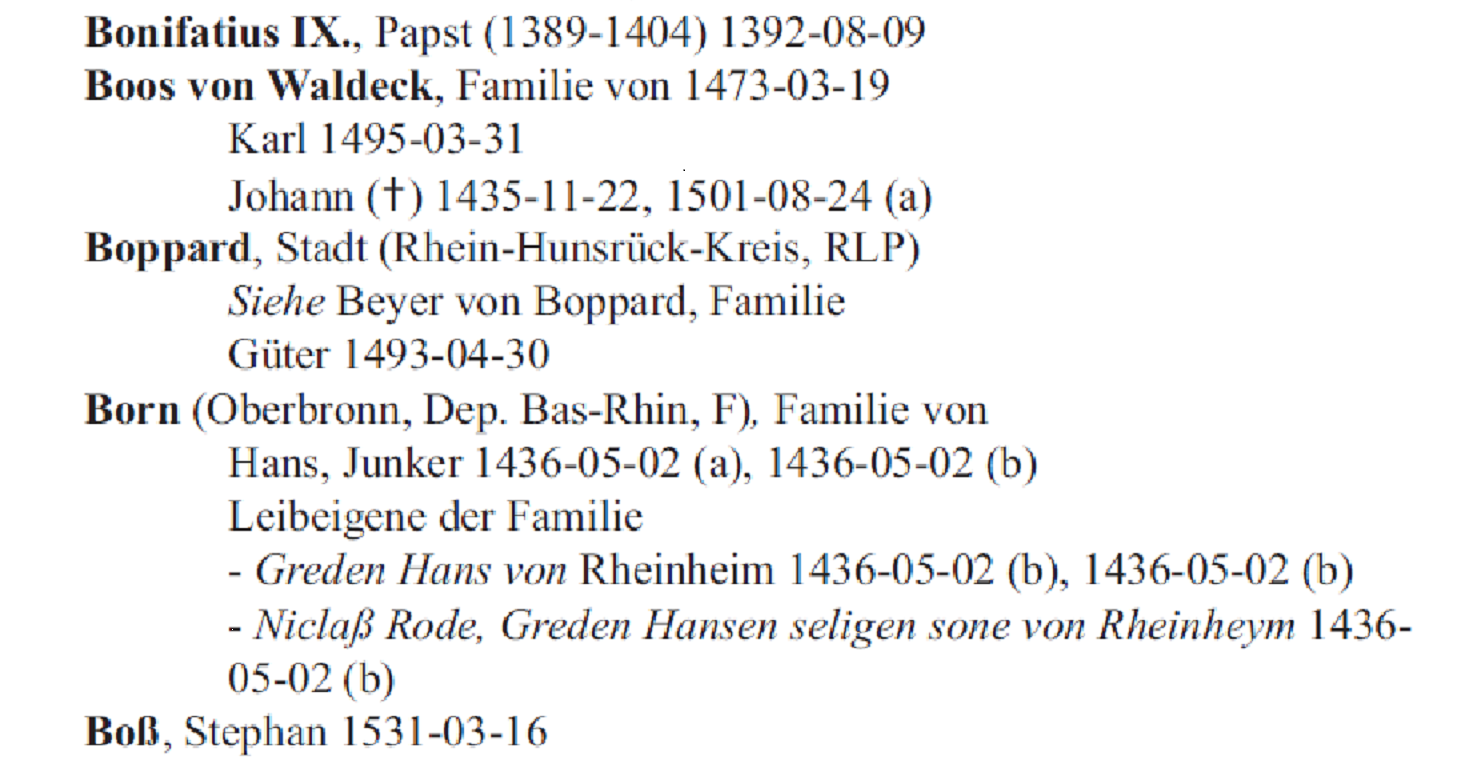
\includegraphics[scale=0.3]{img/index-examples}
  \caption{Examples for index entries taken from the pdf}
  \label{fig:index-examples}
\end{figure}
The index is a manually build list of entities that appear in the regests. It is the last part of the book/pdf and is 277 pages long. Figure \ref{fig:index-examples} shows typical index entries taken from the pdf. The index entries differ from each other, but can roughly be divided into the following five groups: \textit{locations, landmarks, persons, families} and \textit{persongroups}. In total, there there are 1035 index entries (see \ref{fig:type-table} for the distribution of groups). 

\begin{figure}[h]
\centering
\begin{tabular}{|l|c|}
\hline
type        & no  \\
\hline
location    & 550 \\
person      & 103 \\
persongroup & 46  \\
family      & 313 \\
landmark    & 22  \\
other       & 1   \\
\hline
sum         & 1035\\
\hline
\end{tabular} 
\caption{Table...}
\label{fig:type-table}
\end{figure}

\subsection{Index Entries}
Each index entry starts with its name/keyword, which is written in bold. An index entry can intuitively be divided into two parts, which we name \textit{header} and \textit{body}. The header gives more details about the entity, e.g. where a location is located, what profession a person has or in which regest to find the entity. The body gives a list of concepts/entities which are in some (sometimes specified) relation to the index entity. For example \textit{Boos von Waldeck} (see figure \ref{fig:index-examples}) would have the header \textit{Boos von Waldeck, Familie von 1473-03-19} and the body 
\textit{Karl 1495-03-31 Johann (†) 1435-11-22, 1501-08-24 (a)}.

Irrespective of the group they belong to, index entries have some elements in common.
The name might be followed by alternative or additional names. These are usually written in italics (meaning that they are original text) and in parenthesis right after the name. The header of index entries usually ends with a set of numbers in the form of dates, which refer to the particular regests, where this entity is named. Right after these regest-references, there might appear references to other index entities and start with the word \textit{siehe} (\textit{see}).
The body of an index entry is a list of concepts, which are related to the entity. For example \textit{Karl} stands in a relation to the family \textit{Boos von Waldeck}, namely he is a member of it. There exist different layers of such related concepts. If \textit{Karl} had a son for example, he could appear indented below \textit{Karl}. But apparently, a concept on the third level must not obligatorily be in relation with the one the first level. The house where Karl lived could appear below \textit{Karl} as well, although it is not directly related to the family. Often a level is introduced manually between the index entity and body-entities/concepts to group the items. For example Einwohner or Güter, under which there can be found a list of inhabitants/goods which in the regests appeared in relation with the index entity. After each concept there might appear again a set of numbers that refers the reader to the regest, where it appeared.

The part between the name of the entity and the references to the regests is distinct for the different groups. The following sections describe in more detail each of the five groups. 

\begin{figure}[h]
\begin{tabular}{|l|p{9cm}|}
\hline
\textbf{Group}        & \textbf{Possible types}  \\
\hline
location types & Dorf, Stadt, Stadtteil, Burgsiedlung, Burg,  ehem. Burg, Hofgut, Hof, Ort, Örtlichkeit, Gemeinde, Kloster,   Abtei, Schloss, Herrschaft, Herzogtum, Hzgt., Grafschaft,    Gft., Fürstentum, Kgr., Deutschordenskommende, Bistum,     Vogtei, Regierungssitz, Hochstift, Pfarrei, Erzstift, Erzbistum, Dekanat, Domstift, Reichsland, Deutschordensballei,Wasserburg, Mühle, Zisterzienserabtei, Region \\
\hline
landmark types & Berg, Gau, Talschaft, Bach, Tal, Landschaft, Au, Waldung, Wald, Gemeindewald \\
\hline
persongroups   & Notare, Grafen, Markgrafen, Herzöge, Bischöfe, Edelknechte, Herrn von, Herren, Fürsten, Personen, Könige, Ritter von, Einwohner, Päpste, Wildgrafen, Dominikaner \\

\hline
\end{tabular} 
\caption{Types for locations, landmarks and persongroups found in the index.}
\label{fig:location-list}
\end{figure}

\paragraph{Locations}
The locations found in the index are geographical or political. They might also be buildings. Among them are towns, castles, parishes, kingdoms or mills. A full list of the types of locations found in the index can be found in figure \ref{fig:location-list}. They are usually specified in the index entry, right after the name or eventual additional names. They are often followed by districts (Gemeinde, Stadt, Stadtverband, Kreis), regions (Province, Bundesland or Departement) and/or country. Most of the locations are in Germany. The country is only specified, when the location is not in Germany. Sometimes additional descriptions of where to find the location can be found right after the type name (e.g. Dorf im Köllertal, Hof bei St. Ingbert). Locations also specify if a location is no longer inhabited. Entries of such abandoned villages (\textit{Wüstungen}) contain references where to find them in Staerk's catalogue\footnote{Dieter Staerk, Die Wüstungen des Saarlandes, Minerva-Verlag, Saarbrücken, 1974.}). See figure \ref{fig:location-example} for sample entries.

\begin{figure}[h]
  \centering
  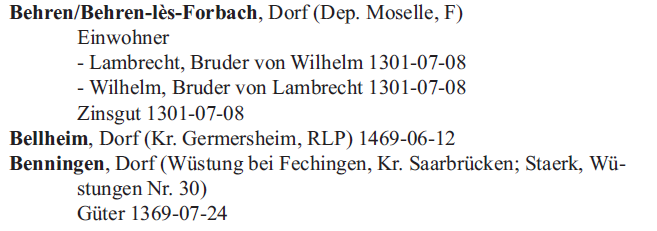
\includegraphics[scale=0.45]{img/location-example}
  \caption{Examples for location index entries taken from the pdf.}
  \label{fig:location-example}
\end{figure}

\paragraph{Landmarks}
Landmarks(equivalent to German \textit{Flurnamen}) are geographical units as forests, mountains, valleys. For the whole list of landmarks found in the index, see figure \ref{fig:location-list}. Landmarks do not provide any additional unique information. See figure \ref{fig:landmark-example} for sample entries.

\begin{figure}[h]
  \centering
  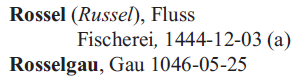
\includegraphics[scale=0.45]{img/landmark-example}
  \caption{Examples for landmark index entries taken from the pdf.}
  \label{fig:landmark-example}
\end{figure}

\paragraph{Persons}
Person-headers may contain forenames, surnames, maiden names, generational names (such as Senior, the first, II.). Additionally they can specify the role or occupation of the person, biographical information such as date of birth or date of the beginning of an important role and relations to other persons (e.g. married with, son of). See figure \ref{fig:person-example} for sample entries.
\begin{figure}[h]
  \centering
  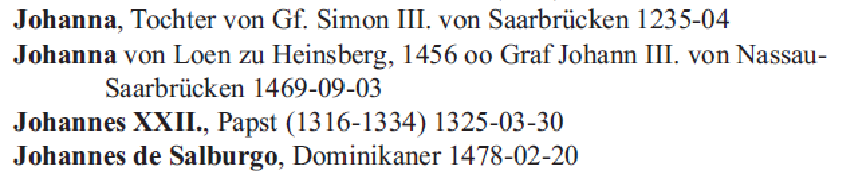
\includegraphics[scale=0.45]{img/person-example}
  \caption{Examples for person index entries taken from the pdf.}
  \label{fig:person-example}
\end{figure}

\paragraph{Families}
Family-headers have no special elements. But their body can be defined more precisely. They do not only represent a list of related entities/concepts, but they are a list of the members of the family. Each of them again might be followed by the regest where it appeared, and at the next level there might appear concepts related to that specific family member. This might again be a family member but not necessarily.
See figure \ref{fig:family-example} for sample entries.

\begin{figure}[h]
  \centering
  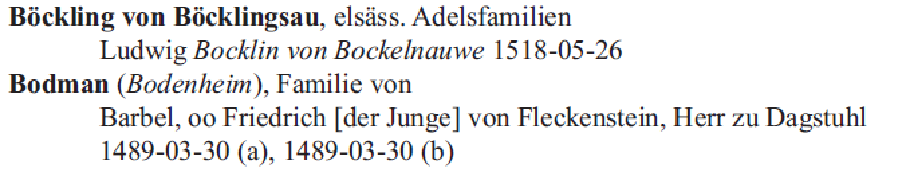
\includegraphics[scale=0.45]{img/family-example}
  \caption{Examples for family index entries taken from the pdf.}
  \label{fig:family-example}
\end{figure}

\paragraph{Persongroups}
Persongroups are index entries that contain a list of people. For example, there is a list for popes, for inhabitants of Saarbrücken, bishops etc. The whole list is shown in figure \ref{fig:location-list}. 
Similar to the families the body is list of concepts which can be specified more concretely. In the case of persongroups, each concept on the first level of the body is a person and so-to-speak member of the group. See figure \ref{fig:persongroup-example} for sample entries.

\begin{figure}[h]
  \centering
  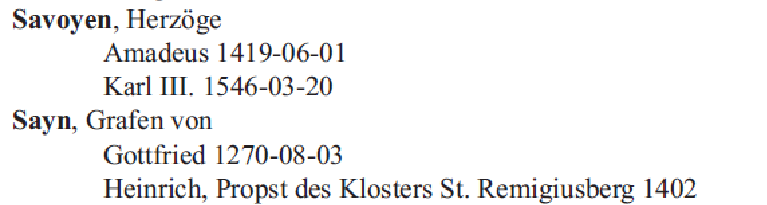
\includegraphics[scale=0.45]{img/persongroup-example}
  \caption{Examples for persongroup index entries taken from the pdf.}
  \label{fig:persongroup-example}
\end{figure}

\paragraph{Others}
Only one index entry is very non-typical and does not fit in any of the proposed groups. It is the entry \textit{Saarbrücken, Gliederung}, which shows an overview over the Saarbrücken entry (see figure \ref{fig:sb-gliederung}). The Saarbrücken entry is the largest index entry with almost 100 pages. It is therefore split up into seven entries, Saarbrücken, Gliederung giving an overview over them.

\begin{figure}[h]
  \centering
  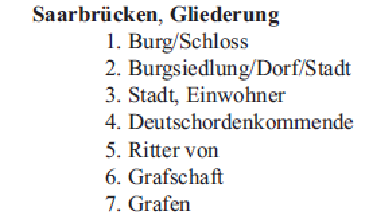
\includegraphics[scale=0.6]{img/sb-gliederung}
  \caption{The index entry \textit{Saarbrücken, Gliederung}.}
  \label{fig:sb-gliederung}
\end{figure}


\subsection{XML Schema for the Index}

One of the main contributions of the Sbr-regesten project was to create an XML schema for the Sbr-regesten. The schema can be found in the file \texttt{sbr-regesten.xsd}.
It was as far as it was applicable designed to comply with the TEI Guidelines \footnote{TEI P5: Guidelines for Electronic Text Encoding and Interchange by the TEI Consortium, Version 2.0.2, 2012}.This section describes the schema for the index.

The index consists of an index-info (for general information about the index), followed by an unrestricted number of items. These are the single index entries.
Each index entry is an item and either a location, person, landmark, persongroup or family. The schema covers them respectively.

Each index item has (required) the following attributes: 
\begin{itemize}
\item id: a unique id (e.g. item\_381)
\item type: location, landmark, person, family or persongroup
\item value: the name of the item (printed in bold in the pdf)
\end{itemize}

%%\begin{figure}[h]
%%\begin{verbatim}
%%<item id="item_661" type="persongroup" value="Notare">
%%\end{verbatim}
%%\label{fig:placeName}
%%\caption{\textit{item} in TEI vs. \textit{placeName} in the Sbr. Regesten schema.}
%%\end{figure}

An index item consists of an item-header and can also have an item-body. The header might for all header types end with the elements \textit{mentioned-in}, followed by \textit{index-refs}. \textit{Mentioned-in} is of type \textit{mentionings} and contains a sequence of references to the regests. The attribute \textit{regest} specifies the id from the regest it refers to. \textit{Index-refs} contains  a sequence of references to other index entries. The attribute \textit{itemid} contains the id from the index item it refers to. Index-refs are allowed to contain free text to insert key words/indications to make evident to the reader, that these are references to index entries (mostly \textit{siehe}).
The next sections will describe in more detail the elements, that items have depending on their type. They will also provide a marked-up example each header and body type.

\subsubsection{Headers}

\paragraph{Location-Header}
Figure \ref{fig:location-header-xml} and \ref{fig:location-wuest-xml} show examples for location headers. Location headers contain the element \textit{placeName}, which corresponds mostly to TEI's \textit{placeName}. See figure \ref{fig:placeName}for an example for a comparision between both. The Sbr-regesten schema adopts TEI's \textit{settlement}, \textit{district}, \textit{region} and \textit{country}. It introduces two new attributes for the settlement element, aside from \textit{type}. It gets the additional attributes \textit{w} and \textit{w-ref} to encode information about abandoned villages (\textit{Wüstungen}). \textit{W} denotes if the settlement is an abandoned village. In that case \textit{w-ref} encodes the reference to the catalogue of Staerk \footnote{Dieter Staerk, Die Wüstungen des Saarlandes, Minerva-Verlag, Saarbrücken, 1974.}. Region types may be \textit{Bundesland} (if located in Germany), \textit{Departement} (in France) or \textit{Province} (Belgium). \textit{Country} has no attribute. TEI defines a \textit{district} as “any kind of subdivision of a settlement, such as a parish, ward, or other administrative or geographic unit.”\footnote{TEI P5: Guidelines for Electronic Text Encoding and Interchange by the TEI Consortium, Version 2.0.2, 2012} In contrast, in our index-locations a \textit{district} is any administrative unit below a \textit{region} (Kreis, Gemeinde, Stadtverband).
Additional to the elements proposed by TEI, the index schema for locations has two more elements: \textit{additional names} (which contains a list of additional names of the location) and \textit{reference-point}, which contains further information not covered by\textit{ district/region/country}. This information specifies where to find the location, e.g. \textit{Im Köllertal, bei St. Ingbert} (in the Köllertal, near St. Ingbert). All of the elements are optional (even settlement, as it also appears in the family headers, where \textit{locations/placeNames} are given, without their names being explicitly specified.)   

\begin{figure}[H]
\begin{verbatim}
<location-header>
   <placeName>
      <settlement type="Dorf" w="false">Frauenberg</settlement>
      <addNames> (
         <addName>Frauwenberg</addName>)
      </addNames>, Dorf (
      <region type="Departement">Dep. Moselle</region>, 
      <country>F</country>) 
   </placeName>
   <mentioned-in>
      <reg-ref regest="regest_235">1452-12-26</reg-ref>, 
      <reg-ref regest="regest_984">1459-02-19</reg-ref>
   </mentioned-in> siehe 
   <index-refs>
      <index-ref itemid="item_534">Lenterdingen</index-ref>,
      <index-ref itemid="item_956"> Volkersweiler</index-ref>
   </index-refs>
</location-header>
\end{verbatim}
\label{fig:location-header-xml}
\caption{Sample \textit{location-header} xml.}
\end{figure}

\begin{figure}[H]
\begin{verbatim}
<location-header>
   <placeName>
      <settlement type="Dorf" w="true" w-ref="Staerk, Wüstungen Nr. 19">
         Arschofen</settlement>
      <ddNames> (
         <addName>Arßhoffen</addName>)
      </addNames>, Dorf 
      <reference-point>im Köllertal</reference-point> (Wüstung, 
      <district>Gde. Gersweiler, Stadtverband Sb.</district>, 
      <region type="Bundesland">SL</region>; Staerk, Wüstungen Nr. 19) 
   </placeName>
</location-header>
\end{verbatim}
\label{fig:location-wuest-xml}
\caption{Sample \textit{location-header} xml with \textit{Wüstung}.}
\end{figure}

\begin{figure}[H]
\begin{verbatim}
<placeName>
    <settlement type="city">Rochester</settlement>,
    <region type="state">New York</region>
</placeName>

<placeName>
    <settlement type="Stadt" w="false">Saarbrücken</settlement>,
    <region type="Bundesland">SL</region>
</placeName>
\end{verbatim}
\label{fig:placeName}
\caption{\textit{placeName} in TEI vs. \textit{placeName} in the Sbr. Regesten schema.}
\end{figure}


\paragraph{Landmark-Header}
Figure \ref{fig:landmark-header-xml} shows an example for a \textit{landmark-header}. Landmark-headers consist of the elements \textit{geogName}, \textit{mentioned-in} and \textit{index-refs}. The element \textit{geogName} is alluded to the TEI \textit{geogName}, but contains exactly the two elements name and \textit{addNames} (additional names).

\begin{figure}[H]
\begin{verbatim}
<landmark-header>
   <geogName type="Fluss">
      <name>Rossel </name>
         <addNames>(
         <addName>Russel</addName>)
      /addNames>
   </geogName>, Fluss 
</landmark-header>
\end{verbatim}
\label{fig:landmark-header-xml}
\caption{Sample for \textit{landmark-header}.}
\end{figure}

\paragraph{Person-Header}
Figure \ref{fig:person-header-xml} shows an example for a person-header. Person headers provide the element \textit{person}. Person consists of \textit{persName} and \textit{description}, where \textit{persName} is very close to TEI's \textit{persName}. It contains (optional) \textit{forename}, \textit{surname}, \textit{genName} (generational name, such as Senior, the first, II., etc., see TEI) and \textit{roleName} (name of the role/occupation? of the person: Fürst, Herzog, Papst, official title/rank/position, see TEI). The only addition to TEI in \textit{persName} is \textit{maidenname} (maiden name). Also here we do not have a single additional name (\textit{addName}), but the element \textit{addNames}, which contains a list off addName elements. It is also important to know that a person has not only an item id (as the other headers do), but also an id that refers to the person itself. This is due to the fact, that the person element is also used in the listing-body. A person therefore has two attributes: \textit{id} and \textit{itemid}.
The other element of person is called description. It provides additional information about the person, such as occupation, relation to other persons (married to, son of, etc.). It is of type content, which means, that it can contain quotes, if the description is taken directly from original text.

\begin{figure}[H]
\begin{verbatim}
<person-header>
   <person id="person_412">
      <persName>
         <forename>Johann</forename> 
         <genName>I.</genName>, 
         <roleName>Graf</roleName>
      </persName>
     <description> von Saarbrücken-Commercy (1307-1341), 
                    oo Mathilde von Apremont    </description>
   </person>
   <mentioned-in>
      <reg-ref regest="regest_543">1310</reg-ref>, 
      <reg-ref regest="regest_1353">1310-10-21</reg-ref>, 
   </mentioned-in>
</person-header>
\end{verbatim}
\label{fig:person-header-xml}
\caption{Sample for \textit{person-header}.}
\end{figure}

\paragraph{Family-Header}
Figure \ref{fig:family-header-xml} shows an example for a family header. Family headers consist of the elements \textit{family-name}, \textit{location}, \textit{mentioned-in} and \textit{index-refs}. \textit{Family-name} consists of name and \textit{addNames} (additional names). Location is of type placeName, which is the same type that location-headers have. See section \textit{location-header} for more details.

\begin{figure}[H]
\begin{verbatim}
<family-header>
  <family-name>
     <name>Brandscheid</name>
     <addNames>
        <addName>Brandscheidt<addName>       
     </addNames>
  </family-name> (
  <location>
     <district>Kr. Bitburg-Prüm</district>, 
     <region type="Bundesland">RLP</region>
  </location>), Familie von 
</family-header>
\end{verbatim}
\label{fig:family-header-xml}
\caption{Sample for \textit{family-header}.}
\end{figure}

\paragraph{Persongroup-Header}
Figure \ref{fig:persongroup-header-xml} shows an example for a persongroup header. Persongroup headers consist of the elements \textit{group-name}, \textit{mentioned-in} and \textit{index-refs}. Group-name is a string, containing the name of the persongroup.
not TEI's \textit{listperson}, because it would be the actual list, which in our case is in the body..

\begin{figure}[H]
\begin{verbatim}
<persongroup-header>
   <group-name>Notare </group-name>
</persongroup-header>
\end{verbatim}
\label{fig:persongroup-header-xml}
\caption{Sample for \textit{persongroup-header}.}
\end{figure}

\subsubsection{Bodies}
There are two different types of bodies: \textit{Concept-body} and \textit{listing-body}.

\paragraph{Concept-body}
TODO: A concept-body contains related concepts. Each related concept consists of at least one concept or person (either only concepts or only persons)
concept:
name
description
mentioned-in
related-concepts
person
see person-header-person
We might also find other concepts in relation to the first lever member.
\begin{figure}[H]
\begin{verbatim}
<concept-body>
   <related-concepts>
      <concept>
         <name> Einwohner </name>
         <related-concepts> -
            <concept>
               <name> Hans gen. Phennewert </name>
               <mentioned-in>
                  <reg-ref regest="regest_64">1455-11-24</reg-ref>
               </mentioned-in>
            </concept> -
            <concept>
               <name> Philipps Pfenwert von Hermanßhusen</name>
               <description>, Bürger zu Saarbrücken, oo Ursulla </description>
               <mentioned-in>
                  <reg-ref regest="regest_756">1510-11-09</reg-ref>, 
                  <reg-ref regest="regest_834">1521-12-24</reg-ref>
               </mentioned-in>
            </concept>
         </related-concepts>
      </concept>
      <concept>
         <name> Güter </name>
         <mentioned-in>
            <reg-ref regest="regest_43">1296-12-29</reg-ref>
         </mentioned-in>
      </concept>
   </related-concepts>
</concept-body>
\end{verbatim}
\label{fig:concept-body-xml}
\caption{Sample for \textit{concept-body}.}
\end{figure}

\paragraph{Listing-body}
Figure \ref{fig:listing-body-xml} shows an example for a \textit{listing-body}. A listing-body consist of the element \textit{members}. \textit{Members} consists of a list of persons (same type as the persons appearing in a person-header). Each person can have related concepts, which recursively can have related concepts again, as in a concept-body.
That means, that in a \textit{persongroup} or \textit{family}, the first layer displays members of that family or group. The concepts on the levels beyond might also be family or group members but not obligatory. Therefore they are not modelled as members on their own, but as related-concepts of that member.

\begin{figure}[H]
\begin{verbatim}
<listing-body>
  <members>
     <person id="person_89">
        <persName>
           <forename> Dietrich </forename>gen.
           <addNames>
              <addName> Gebürghin </addName>
           </addNames>
        </persName>
        <mentioned-in>
           <reg-ref regest="regest_823">1460-12-01</reg-ref>
        </mentioned-in>
        <related-concepts> -
           <concept>
              <name> Knecht Peter </name>
              <mentioned-in>
                 <reg-ref regest="regest_823">1460-12-01</reg-ref>
              </mentioned-in>
           </concept>
        </related-concepts>
     </person>
     <person id="person_90">
        <persName>
           <forename> Jakob von Brandscheid</forename>
        </persName>
        <description>, Amtmann zu Saargemünd </description>
        <mentioned-in>

           <reg-ref regest="regest_934">1519-03-23</reg-ref>
        </mentioned-in>
     </person>
  </members>
</listing-body>
\end{verbatim}
\label{fig:listing-body-xml}
\caption{Sample for \textit{listing-body}.}
\end{figure}


\subsection{Index Extraction}
In order to convert the Sbr-regesten into an XML, relevant pieces of information have to be extracted from the pdf and tagged according to the schema. Additionally, the regests and index entries are written into the database \texttt{sbr-regesten.db}.

\paragraph{From PDF to HTML}
In order to extract information from the Sbr-regesten, the structural information an HTML provides, is very useful. Apart from the .pdf file the publishers provided us with a .doc version of the Sbr-regesten. Using Microsoft Word 2010, it is possible to store the document as HTML. Compared to different tools, we tried out, it was the most useful version we could extract. The extracted HTML is the one we use for the extraction.
As there arose some minor difficulties where the HTML was inconsistent, we manually manipulated it (TODO).
The extracted HTML file \texttt{html/sbr-regesten.hmtl} is used for the extraction of all parts of the book.

This chapter will describe in more detail how the XML for the index is extracted. Figure (TODO) gives an overview over the index\_extractor.
The index\_extractor is divided into three parts

\begin{itemize}
\item index\_to\_xml converts the HTML to an almost complete XML
\item index\_xml\_postprocess solves the references to the index entries and adds them to the XML
\item index\_to\_db extracts the index-items from the XML and writes them into the database
\end{itemize}

The separation of converting the index into XML and writing them into the database, has two reasons: it is easier structured and it is possible to manually correct the XML-file before adding the items into the database.

\subsubsection{From the Index to the XML}
ItemExtractor
The extraction of the single index items is very staightforward, as the HTML provides tags for paragraphs (<p>). Each index item is a paragraph. Once the ItemExtractor identified a paragraph, it instantiates an index item, and divides the HTML into header and body.

ItemClassifier
With the help of a set of names/keys (retrieved by bootstrapping), each item is assigned to a group (location, landmark, person, family, persongroup, siehe) and forwarded to the corresponding parser. The items stored in the "siehe" Liste contain no direct information about the group they belong to. But they contain references to other index entry. Assuming that they have the same type, they are forwarded to the corresponding parser after having solved the reference. Items that do not contain any of the keywords are stored in the list "unclassified" and are not further processed. This is the case for the \textit{Saarbrücken, Gliederung} entry.

ItemParser
There is an item parser for each of the five groups. It forwards the header to the specific header parser of its group and the body to one of the two body parsers. It then adds the item to an itemList.


\subsubsection{From the Index XML to the Database}
TODO: This section presents possible next steps. Depending on the use or queries of the Sbr-regesten, different expansions will have priority

\subsubsection{Future Work}
\paragraph{References to the Regests}
At the time of developing the index extraction, the regest part of the book was not extracted or written into the database yet. Once this is the case, the first expansion of the current code would be to solve the references to the regests. The references are already recognised and tagged with reg-ref. Each reg-ref is supposed to store the id of the regest it refers to in the attribute regest. At the moment, this is not yet the case. The function \texttt{get\_regest\_ID} in \texttt{index\_to\_xml.py} returns the correct id only in cases where the date in the form "1532-11-24" is sufficient to disambiguate the regests. In other cases it returns the dummy id regest\_99999. We would recommand to reimplement the function \texttt{get\_regest\_ID} and solve the references directly searching the database, as the regests are added to the database before \texttt{index\_to\_xml.py} is called. To include the references also in the database, the function def \texttt{ment\_to\_db} in \texttt{index\_to\_db.py} has to be implemented.

\paragraph{Extracting Person Names}
TODO: The index extractor allows the user to provide a list of forenames (\texttt{resources/forenames.txt}. During the extraction of the index it uses the list to recognize forenames and expands it at the same time. ...
list of forenames as input, postprocess similar to siehe, manually increment list with forenames from other sources. Same would be possible for surnames

\paragraph{Semantic Network}
The regests and the index do not provide only information about entities, but also about the relations they have. This becomes evident especially in the case of persons. The index already provides information such as "married with" or "son of". This information could be extracted to build networks of relations between persons.

\paragraph{Quotes}
The HTML provides information about which parts of the text are original text. Such sections are marked with italics (<i>). To mark original text the Sbr-regesten schema introduces the element 'Quotes'. This is mainly used in the regests. In the index quotes are only possible in the description part of the bodies. The tag <addNames> implicitly encodes this information as they extract text in italics. Otherwise this information gets lost during the process of extraction. But we can imagine the usefulness of conserving information about original text also in other parts of the index, we propose to expand the schema to allow quotes.

\paragraph{Expand References to the Index}
TODO: References to the index are only found and solved if they appear in the header right after the mentionings. But in some cases such references occur in other places as well (often in the bodies or before the district). The schema could be adapted to allow "reg-refs" there as well. They would have to be marked by texttt{index\_to\_xml.py} and would then (automatically) be extracted by the existing the \texttt{parse\_siehe} function in \texttt{index\_xml\_postprocess}.